\documentclass{beamer}  
%导言区
%\usepackage[UTF8,noindent]{ctexcap}%阻止ctex宏包引入的短浅缩进
\usetheme{AnnArbor}
\usepackage{graphicx}
%set equation theme
\setbeamertemplate{footline}[frame number]{}
\usefonttheme{professionalfonts}
\usepackage{algorithm2e}
\usepackage{algorithmic}
\usepackage[level]{datetime} 
\usepackage{biblatex}
	\bibliography{BMVC2018}

%set theme
\useinnertheme{rectangles}
\useoutertheme{smoothbars}%sidebar
\usecolortheme{crane}%crane
\begin{document}  
	
%second section 
	
	
	\title{High-Resolution Image Synthesis and Semantic Manipulation with Conditional GANs}
	\institute[SCUT]{South China University of Technology}
	%\logo{
\includegraphics[height=0.45\textwidth]{graphics/scut.pdf}}
	\author{Presented by Junhong Huang}
	\titlegraphic{	
\includegraphics[height=0.35\textwidth]{images/scut.pdf}}
	\date{May 27, 2018, SAIL}
	\keywords{GAN,WGAN,machine learning,deep learning}
	
	%first
	\begin{frame}
	\maketitle
\end{frame}

\begin{frame}{Contents}
%content
\tableofcontents
\end{frame}



\AtBeginSection[]
{
\begin{frame}{Contents}

\tableofcontents[currentsection]

\end{frame}
}

\section{Motivation}
\begin{frame}{Motivation}{High-Resolution Image Synthesis \& Semantic Manipulation }
\begin{figure}
	\centering
	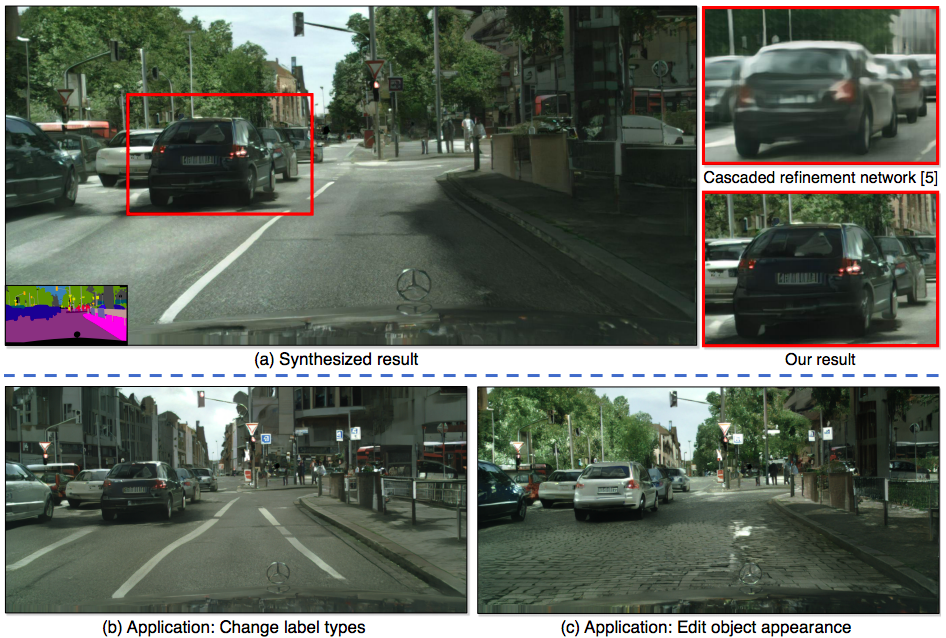
\includegraphics[height=0.5\textheight]{images/conclusion}
%	\caption{$2048\times1024$ images generated from the  semantic label map (lowe left coner in (a))}
\end{figure}
\setbeamercolor{uppercol}{fg=white,bg=blue!75!black}%
\setbeamercolor{lowercol}{fg=black,bg=blue!20}%
\begin{beamerboxesrounded}[upper=uppercol,lower=lowercol,shadow=false]{In this paper,}
	\begin{itemize}
	\item
	high-resolution image synthesis is \textbf{generating $2048\times1024$ photo-realistic images} from semantic label maps;
	\item
	semantic manipulation means allowing users to \textbf{edit the object appearance} interactively.
	\end{itemize}
\end{beamerboxesrounded}
\end{frame}

\section{Method}
\begin{frame}{The pix2pix Baseline \footcite{Image-to-image translation with conditional adversarial networks (CVPR 2017)}}
\begin{figure}
	\centering
	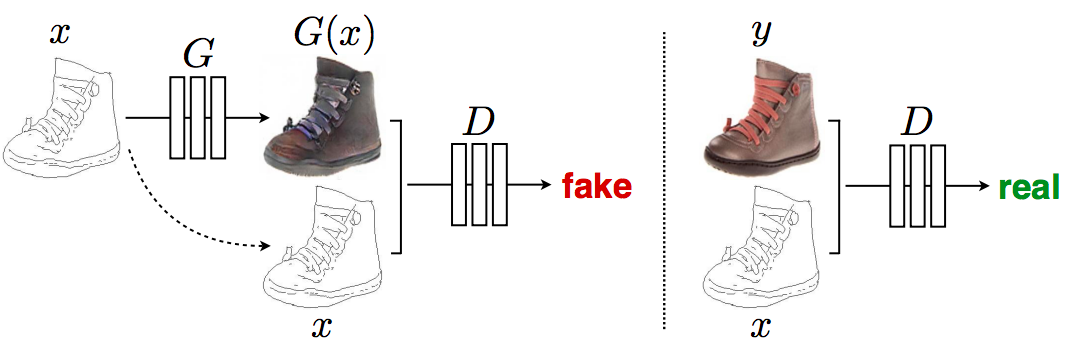
\includegraphics[height=0.4\textheight]{images/baseline}
\end{figure}
\setbeamercolor{uppercol}{fg=white,bg=blue!75!black}%
\setbeamercolor{lowercol}{fg=black,bg=blue!20}%
\begin{beamerboxesrounded}[upper=uppercol,lower=lowercol,shadow=false]{The Value Function}
\begin{equation}
\begin{aligned}
	\mathcal{L}_{cGAN}(G,D)=&\mathbb{E}_{x,y}[\log D(x,y)]\\+&\mathbb{E}_{x,z}[\log(1-D(x,G(x,z)))]
\end{aligned}
\end{equation}
\end{beamerboxesrounded}
\end{frame}

\begin{frame}{The pix2pix Baseline }
\begin{figure}
	\centering
	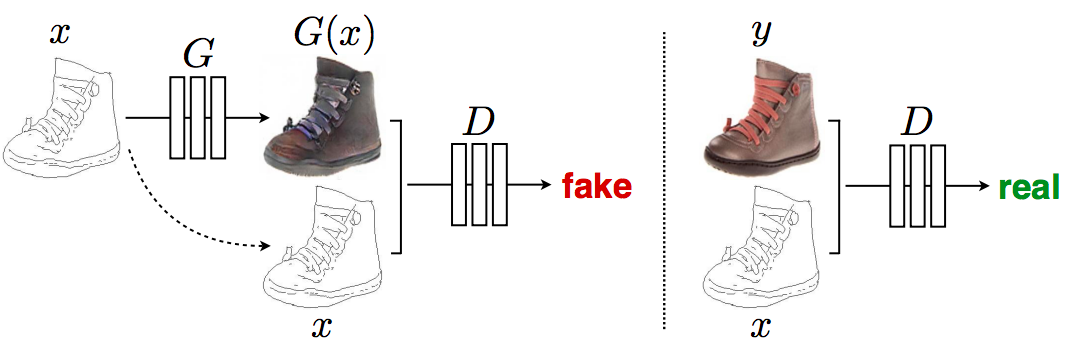
\includegraphics[height=0.4\textheight]{images/baseline}
\end{figure}
\setbeamercolor{uppercol}{fg=white,bg=red!75!black}%
\setbeamercolor{lowercol}{fg=black,bg=red!20}%
\begin{beamerboxesrounded}[upper=uppercol,lower=lowercol,shadow=false]{Existing problems in this baseline}
\begin{itemize}
	\item
	The resolution of the generated images is \textbf{up to $256\times256$};
	\item 
	When we use it to generate high-resolution images, its \textbf{training is unstable}, and \textbf{the quality of results is unsatisfactory}.
\end{itemize}
\end{beamerboxesrounded}
\end{frame}

\begin{frame}{Improving Photorealism and Resolution}{Coarse-to-Fine Generator}
	\begin{figure}
	\centering
	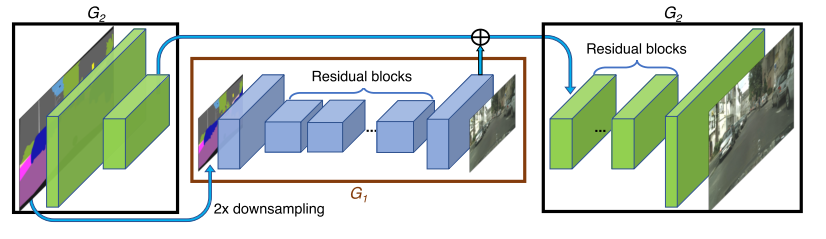
\includegraphics[height=0.4\textheight]{images/structure}
\end{figure}
\setbeamercolor{uppercol}{fg=white,bg=blue!75!black}%
\setbeamercolor{lowercol}{fg=black,bg=blue!20}%
\begin{beamerboxesrounded}[upper=uppercol,lower=lowercol,shadow=false]{Details}
\begin{itemize}
	\item
	Global generator $G_1$: $1024\times512$ (resolution)
	\item
	Local generator $G_2$: $2048\times1024$ (resolution)
\end{itemize}
\end{beamerboxesrounded}
\end{frame}

\begin{frame}{Improving Photorealism and Resolution}{Multi-scale  Discriminators}
	\begin{figure}
	\centering
	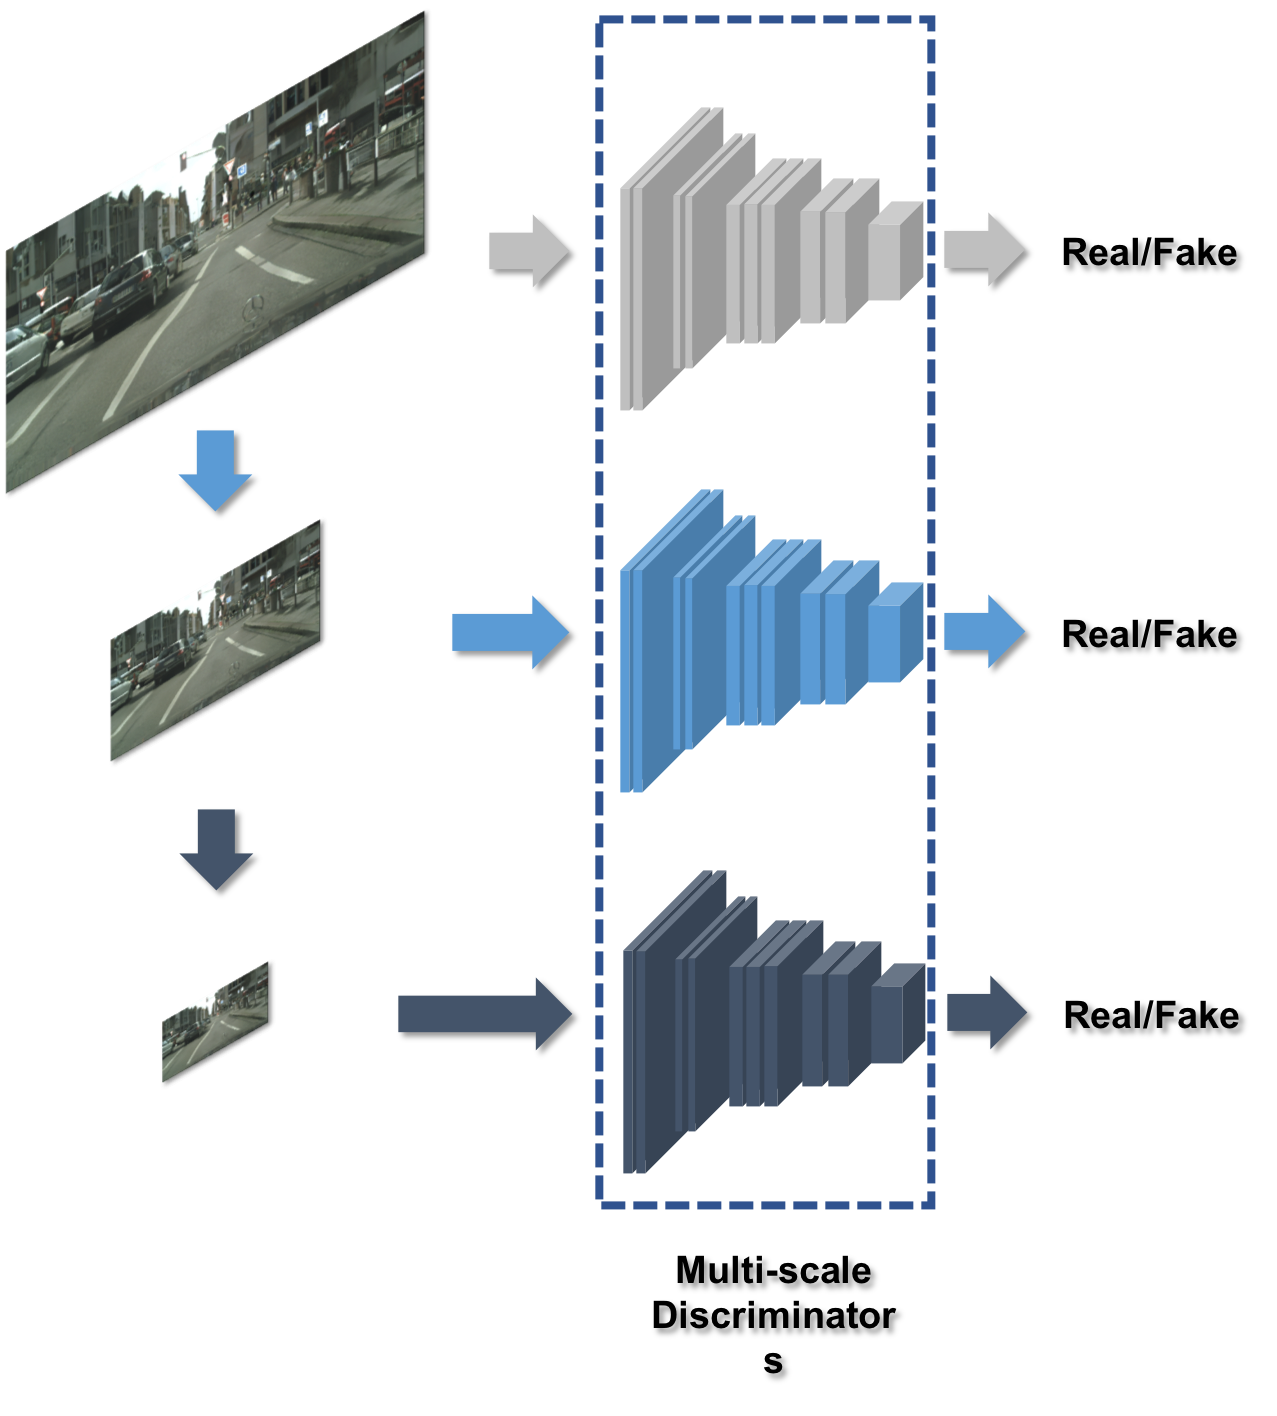
\includegraphics[height=0.6\textheight]{images/multi-scale}
\end{figure}
\setbeamercolor{uppercol}{fg=white,bg=blue!75!black}%
\setbeamercolor{lowercol}{fg=black,bg=blue!20}%
\begin{beamerboxesrounded}[upper=uppercol,lower=lowercol,shadow=false]{Modified GAN Loss}

\begin{equation}
\min_G\max_{D_1,D_2,D_3}\sum_{k=1,2,3} \mathcal{L}_{GAN}(G,D_k)
\end{equation}
\end{beamerboxesrounded}

\end{frame}

\begin{frame}{Improving Photorealism and Resolution}{Improved Adversarial Loss and Full Objective}

	Improved adversarial loss:
	\begin{equation}
	\mathcal{L}_{FM}(G,D_k)=\mathbb{E}_{(s,x)} \sum_{i=1}^T \frac{1}{N_i}[||D_k^{(i)}(s,x)-D_{k}^{(i)}(s,G(s))||_1]
	\end{equation}
	The full objective:
	\begin{equation}
\min_G ((\max_{D_1,D_2,D_3}\sum_{k=1,2,3} \mathcal{L}_{GAN}(G,D_k)))+\lambda \sum_{k=1,2,3}\mathcal{L}_{FM}(G,D_K)
	\end{equation}
\end{frame}

\begin{frame}{Using Instance Maps}
\begin{figure}
	\centering
	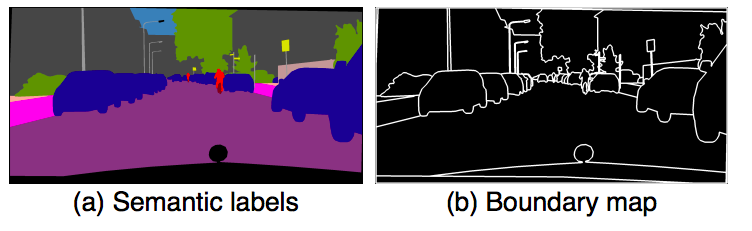
\includegraphics[height=0.45\textheight]{images/instance_maps}
\end{figure}
\setbeamercolor{uppercol}{fg=white,bg=blue!75!black}%
\setbeamercolor{lowercol}{fg=black,bg=blue!20}%
\begin{beamerboxesrounded}[upper=uppercol,lower=lowercol,shadow=false]{Implementation }
A pixel in the instance boundary map is 1 if its object ID is different from any of its 4-neighbors, and 0 otherwise.
\end{beamerboxesrounded}
\end{frame}

\begin{frame}{Using Instance Maps}
\begin{figure}
	\centering
	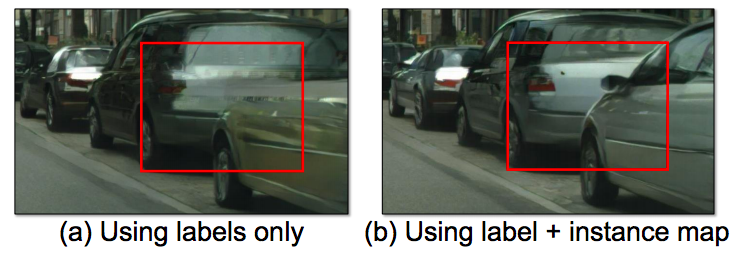
\includegraphics[height=0.45\textheight]{images/instance_result}
\end{figure}
\end{frame}

\begin{frame}{Learning an Instance-level Feature Embedding}
\begin{figure}
	\centering
	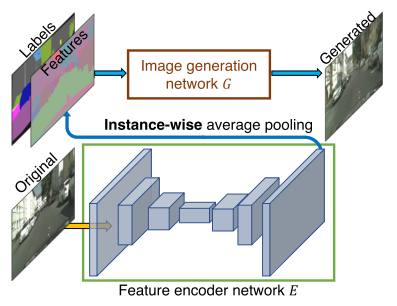
\includegraphics[height=0.5\textheight]{images/instance}
\end{figure}
\setbeamercolor{uppercol}{fg=white,bg=blue!75!black}%
\setbeamercolor{lowercol}{fg=black,bg=blue!20}%
\begin{beamerboxesrounded}[upper=uppercol,lower=lowercol,shadow=false]{To generate diverse images \& allow instance-level control, }
\begin{itemize}
	\item
	train a encoder network $E$ (replace $G(s)$ with $G(s,E(x))$)
	\item
	record the obtained features of all instances.
	\item
	do K-means clustering 
	\item
	resent K modes for users (K cluster centers)
	
	\end{itemize}
\end{beamerboxesrounded}
\end{frame}







\section{Experimental Results}
\begin{frame}{Datasets and Baselines}
\setbeamercolor{uppercol}{fg=white,bg=blue!75!black}%
\setbeamercolor{lowercol}{fg=black,bg=blue!20}%
\begin{beamerboxesrounded}[upper=uppercol,lower=lowercol,shadow=false]{In this paper, }
	\begin{itemize}
		\item
	datasets include \textbf{Cityscapes}, \textbf{NYU Indoor RGBD}, \textbf{ADE20K} and \textbf{Helen Face} datasets;
		\item
	baselines contain \textbf{pix2pix} \footcite{Image-to-image translation with conditional adversarial networks (CVPR 2017)} and \textbf{CRN} \footcite{Photographic image synthesis with cascaded refinement networks (ICCV 2017)}
	\end{itemize}
\end{beamerboxesrounded}
\end{frame}

\begin{frame}{Quantitative Comparisons }
\begin{figure}
	\centering
	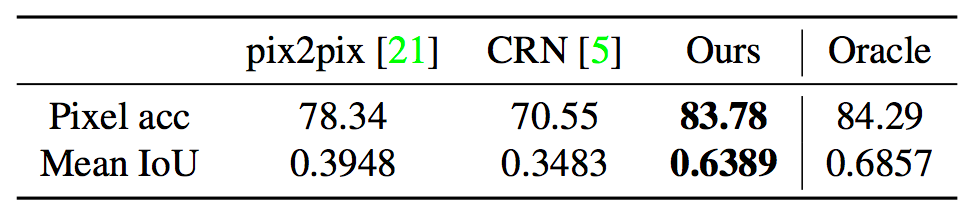
\includegraphics[height=0.25\textheight]{images/table_1}
\end{figure}
\begin{figure}
	\centering
	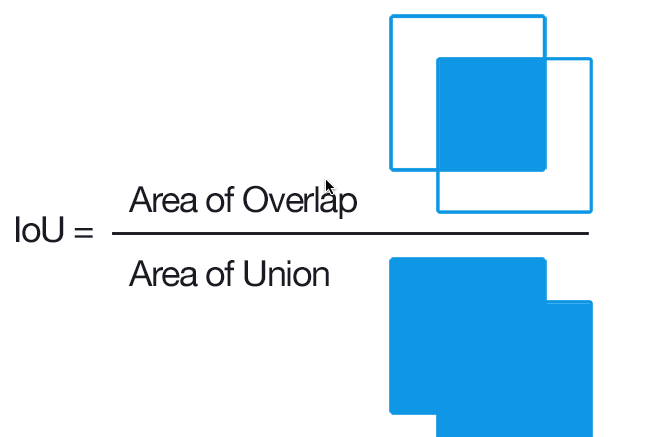
\includegraphics[height=0.25\textheight]{images/IoU}
\end{figure}
\setbeamercolor{uppercol}{fg=white,bg=blue!75!black}%
\setbeamercolor{lowercol}{fg=black,bg=blue!20}%
\begin{beamerboxesrounded}[upper=uppercol,lower=lowercol,shadow=false]{Details }
 PSPNet is used  to predict the ground true label map with the generated photo-realistic images.
\end{beamerboxesrounded}

\end{frame}


\begin{frame}{Human Perceptual Study}{Unlimited Time}
\begin{figure}
	\centering
	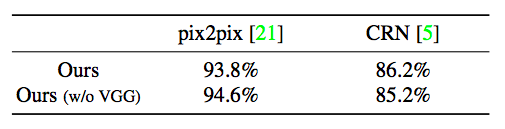
\includegraphics[height=0.35\textheight]{images/unlimite_time}
\end{figure}
\setbeamercolor{uppercol}{fg=white,bg=blue!75!black}%
\setbeamercolor{lowercol}{fg=black,bg=blue!20}%
\begin{beamerboxesrounded}[upper=uppercol,lower=lowercol,shadow=false]{Details }
Each cell lists the percentage where our result is preferred over the other method.
\end{beamerboxesrounded}
\end{frame}

\begin{frame}{Human Perceptual Study}{Unlimited Time}
\begin{figure}
	\centering
	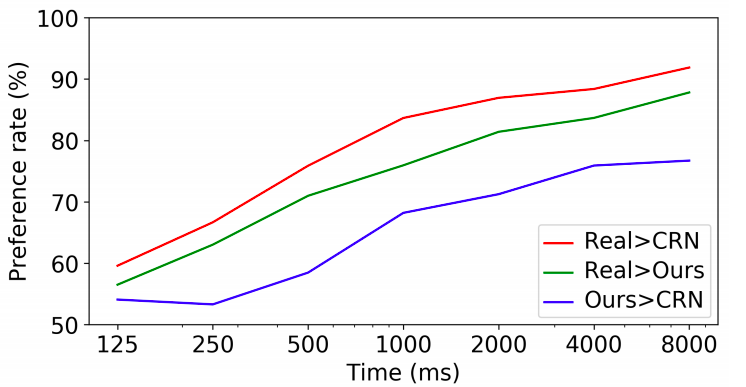
\includegraphics[height=0.45\textheight]{images/limite_time}
\end{figure}
\setbeamercolor{uppercol}{fg=white,bg=blue!75!black}%
\setbeamercolor{lowercol}{fg=black,bg=blue!20}%
\begin{beamerboxesrounded}[upper=uppercol,lower=lowercol,shadow=false]{Details }
The comparison results at \textbf{different time intervals} are shown as aforementioned figure.
\end{beamerboxesrounded}
\end{frame}

\begin{frame}{Analysis of Proposed Model}{Analysis of The Loss Function}
\begin{figure}
	\centering
	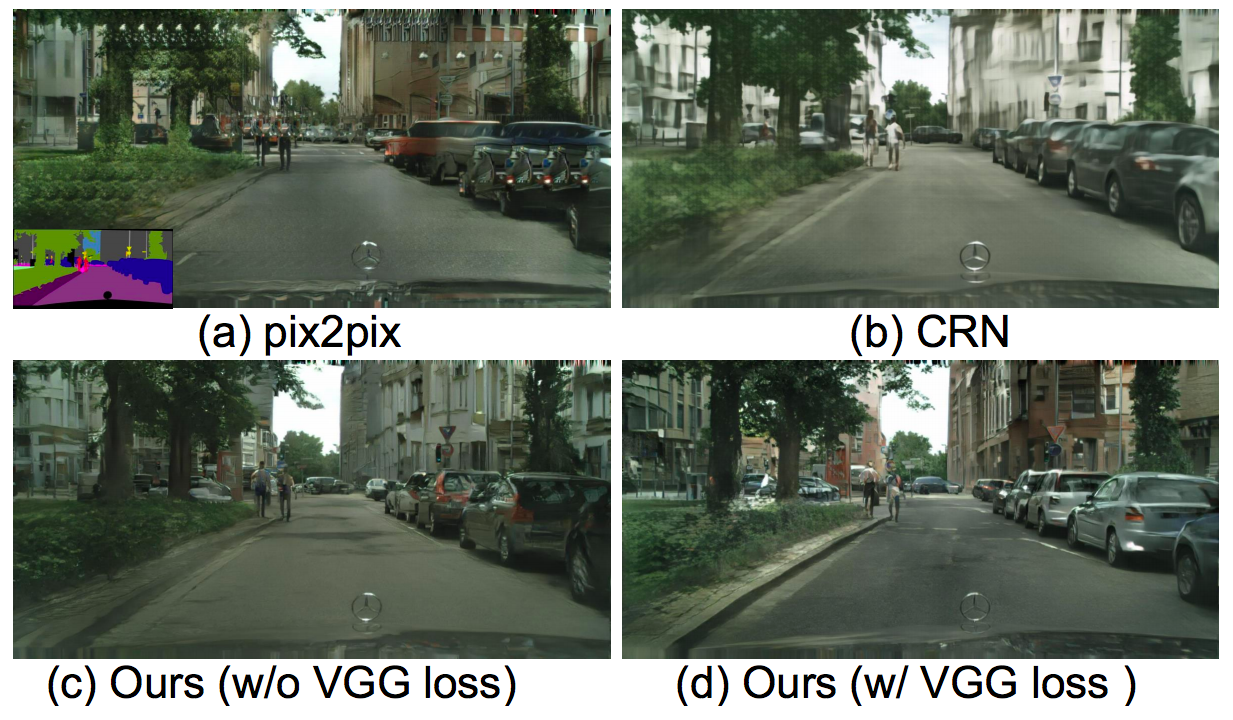
\includegraphics[height=0.8\textheight]{images/result_1}
\end{figure}
\end{frame}


\begin{frame}{Analysis of Proposed Model}{Analysis of The Loss Function}
\begin{figure}
	\centering
	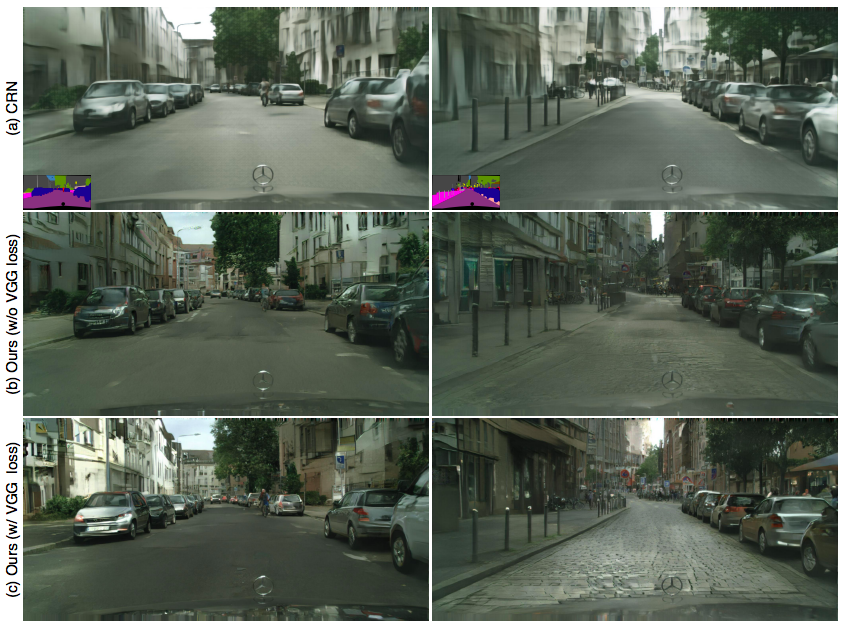
\includegraphics[height=0.8\textheight]{images/result_3}
\end{figure}
\end{frame}

\begin{frame}{Analysis of Proposed Model}{Analysis of  Using Instance Maps}
\begin{figure}
	\centering
	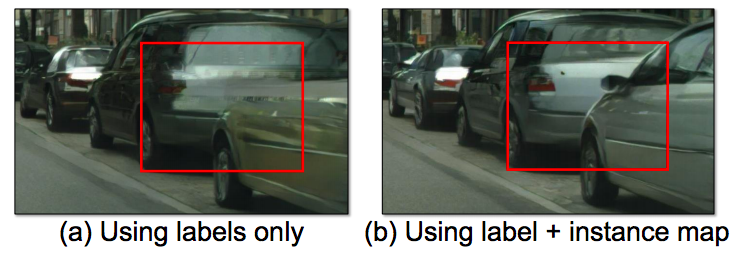
\includegraphics[height=0.45\textheight]{images/instance_result}
\end{figure}
\setbeamercolor{uppercol}{fg=white,bg=blue!75!black}%
\setbeamercolor{lowercol}{fg=black,bg=blue!20}%
\begin{beamerboxesrounded}[upper=uppercol,lower=lowercol,shadow=false]{Comparison }
Using instance maps improves the \textbf{realism} of  results, especially around the object \textbf{boundaries}.
\end{beamerboxesrounded}
\end{frame}

\begin{frame}{Analysis of Proposed Model}{Analysis of  The generator}
\begin{figure}
	\centering
	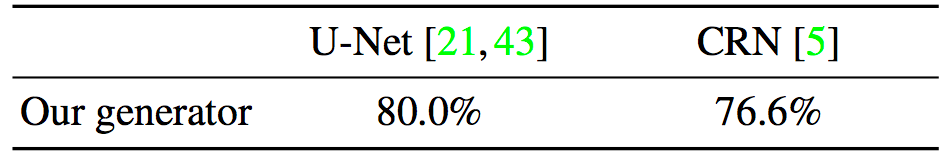
\includegraphics[height=0.2\textheight]{images/table_3}
\end{figure}
\setbeamercolor{uppercol}{fg=white,bg=blue!75!black}%
\setbeamercolor{lowercol}{fg=black,bg=blue!20}%
\begin{beamerboxesrounded}[upper=uppercol,lower=lowercol,shadow=false]{Comparison }
	\begin{itemize}
		\item
Pairwise comparison results on the Cityscapes dataset.
\item
 Each cell lists the percentage where our result is preferred over the other method.
 \end{itemize}
\end{beamerboxesrounded}
\end{frame}

\begin{frame}{Analysis of Proposed Model}{Analysis of The Discriminator}
\begin{figure}
	\centering
	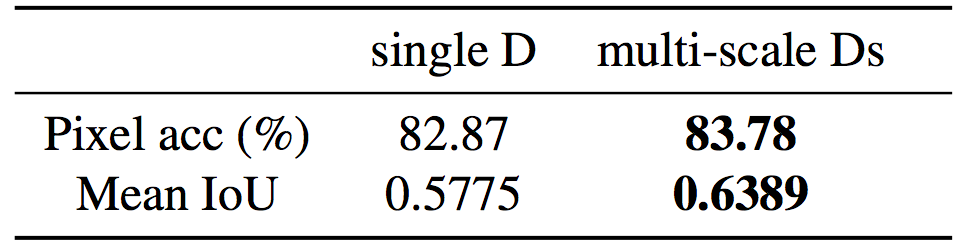
\includegraphics[height=0.3\textheight]{images/table_4}
	\caption{The segmantation scores on Cityscapes dataset.}
\end{figure}

\end{frame}

\begin{frame}{Iterative Object Editing}
\begin{figure}
	\centering
	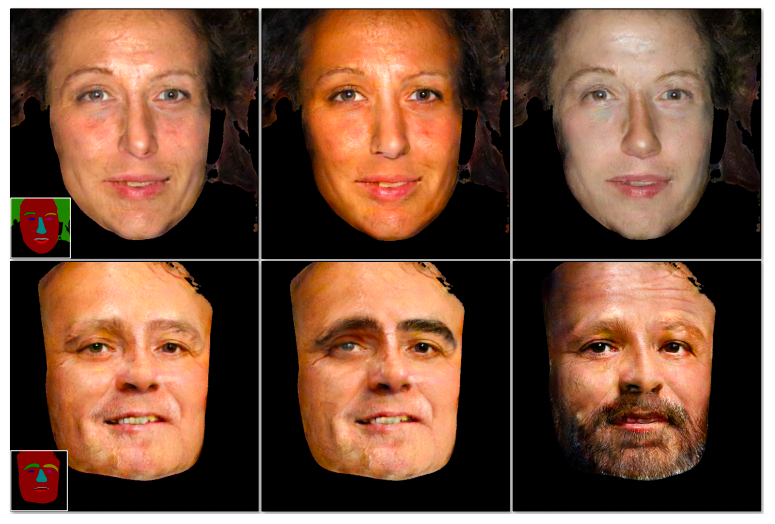
\includegraphics[height=0.6\textheight]{images/result_4}
\end{figure}
\end{frame}







\section{Conclusions}
\begin{frame}{Contributions and Limitations}
\setbeamercolor{uppercol}{fg=white,bg=green!75!black}%
\setbeamercolor{lowercol}{fg=black,bg=green!20}%
\begin{beamerboxesrounded}[upper=uppercol,lower=lowercol,shadow=false]{	Contributions }

\begin{itemize}
	
	\item
	Generate high-resolution photo-realistic images;
	\item
	Allow users to edit the object appearance interactively.
\end{itemize}
\end{beamerboxesrounded}\setbeamercolor{uppercol}{fg=white,bg=red!75!black}%
\setbeamercolor{lowercol}{fg=black,bg=red!20}%


\begin{beamerboxesrounded}[upper=uppercol,lower=lowercol,shadow=false]{	Limitations }

\begin{itemize}
	
	\item
	Some regions in the generated results are still unrealistic;
	\item
	Semantic manipulation method need to be improved.
\end{itemize}
\end{beamerboxesrounded}


\end{frame}

\begin{frame}
\begin{figure}
	\centering
	
\includegraphics[height=0.6\textheight]{images/Theend}
\end{figure}
\end{frame}
\end{document} 